\subsection{MoBAAttention (\texttt{moba\_attention})}
\label{sec:app_module_moba_attention}

\subsubsection*{3.1 Module Overview}
MoBA: Mixture of Block Attention for Long-Context Modeling.
\begin{itemize}
    \item \textbf{Track Paradigm:} Track 3: Mixture-of-Experts \& Dynamic Routing
    \item \textbf{Source File Path:} \texttt{Codes/framework/attentions/moba\_attention.py}
    \item \textbf{Registration Name:} \texttt{moba\_attention} $\mid$ \textbf{Class:} \texttt{MoBAAttention}
\end{itemize}

\subsubsection*{3.2 Mathematical Formulation}
Let $X \in \mathbb{R}^{B \times L \times d_{\text{in}}}$ denote the batch sequence representation tensor for batch size $B$, sequence length $L$, and channel dimension $d_{\text{in}}$. The exact forward mathematical transformation of \texttt{moba\_attention} is formulated as:

\begin{align}
H(x) &= x \cdot W_g \in \mathbb{R}^{E}, \quad G(x) = \operatorname{TopK}\left(\operatorname{softmax}(H(x)), k\right), \\
Y &= \sum_{i \in \operatorname{TopK}} G(x)_i \cdot E_i(x), \quad E_i(x) = \operatorname{GELU}(x W_{1, i}) W_{2, i}.
\end{align}


\subsubsection*{3.3 Computational Complexity}
\begin{itemize}
    \item \textbf{Time Complexity:} $\mathcal{O}(N d \frac{k}{E})$
    \item \textbf{Memory State Complexity:} $\mathcal{O}(E d^2)$
    \item \textbf{Scaling Class:} Decouples active computation $\mathcal{O}(k)$ from total parameter capacity $E$, achieving sub-quadratic execution cost.
\end{itemize}

\subsubsection*{3.4 Key Hyperparameters}
\begin{itemize}
    \item \texttt{config}: Operational hyperparameter.
    \item \texttt{block\_size}: Operational hyperparameter.
    \item \texttt{top\_k}: Operational hyperparameter.
    \item \texttt{rank}: Low-rank compression bottleneck.
\end{itemize}

\subsubsection*{3.5 Empirical Performance Telemetry}
Table~\ref{tab:telemetry_moba_attention} reports the empirical hardware performance measurements recorded on an isolated NVIDIA GeForce RTX 4070 Laptop GPU (8GB VRAM, CUDA 12.4, AMP FP16 enabled, batch size $B=4$, sequence length $L=128$).

\begin{table}[h]
\centering
\small
\caption{\textbf{Empirical Benchmark Telemetry for \texttt{moba\_attention}}. Measured on NVIDIA RTX 4070 Laptop GPU across standard GLUE tasks.}
\label{tab:telemetry_moba_attention}
\begin{tabular*}{\columnwidth}{@{\extracolsep{\fill}}lccccc}
\toprule
\textbf{Model Family} & \textbf{Status} & \textbf{Accuracy} & \textbf{F1-Score} & \textbf{Peak VRAM} & \textbf{Throughput} \\
\midrule
DistilBERT & \texttt{PASS} & 73.62\% & 75.16\% & 329.0 MB & 51,081 tok/s \\
RoBERTa & \texttt{PASS} & 84.17\% & 85.83\% & 379.1 MB & 27,860 tok/s \\
GPT-2 & \texttt{PASS\_LOW} & 50.92\% & 67.48\% & 569.5 MB & 19,829 tok/s \\
Qwen & \texttt{PASS} & 51.95\% & --- & --- & --- \\
Unknown & \texttt{PASS} & 30.87\% & --- & --- & --- \\
\bottomrule
\end{tabular*}
\end{table}

\subsubsection*{3.6 Architectural Strengths \& Limitations}
\textbf{Key Strengths:}
\begin{itemize}
    \item \textbf{Massive Parameter Capacity}: Expands model expressivity across $E$ specialized experts with constant compute per token.
    \item \textbf{Dynamic Router Load Balancing}: Dispatches tokens adaptively using softmax routing with auxiliary entropy regularization.
    \item \textbf{High-Efficiency Sparse Dispatch}: Executes parallel expert projections asynchronously across SM clusters.
\end{itemize}

\textbf{Potential Limitations:}
\begin{itemize}
    \item \textbf{Routing Communication Overhead}: All-to-all token dispatch across distributed nodes can introduce interconnect latency.
    \item \textbf{Expert Imbalance Risk}: Without load-balancing loss, tokens may collapse to a small subset of dominant experts.
    \item \textbf{High VRAM Memory Footprint}: Requires sufficient GPU memory to host all $E$ expert parameter matrices simultaneously.
\end{itemize}

\subsubsection*{3.7 Implementation \& System Notes}
The module \texttt{moba\_attention} is natively integrated into the NeuralOps registry with automated AMP FP16 tensor casting, fused linear down/up-projection passes, and exact autograd backward graph registration. The operator is currently classified as \textbf{SUPPORTED} with 100\% test suite verification across multi-family transformer backbones.

\subsubsection*{3.8 Architectural Characterization Diagram}
Figure~\ref{fig:module_moba_attention} provides the complete 3-panel architectural visualization detailing: (a) Computational Dataflow Graph; (b) Structural Dynamics and Matrix Pattern; and (c) Complexity Scaling Profile against Quadratic Baselines.

\begin{figure}[htbp]
    \centering
    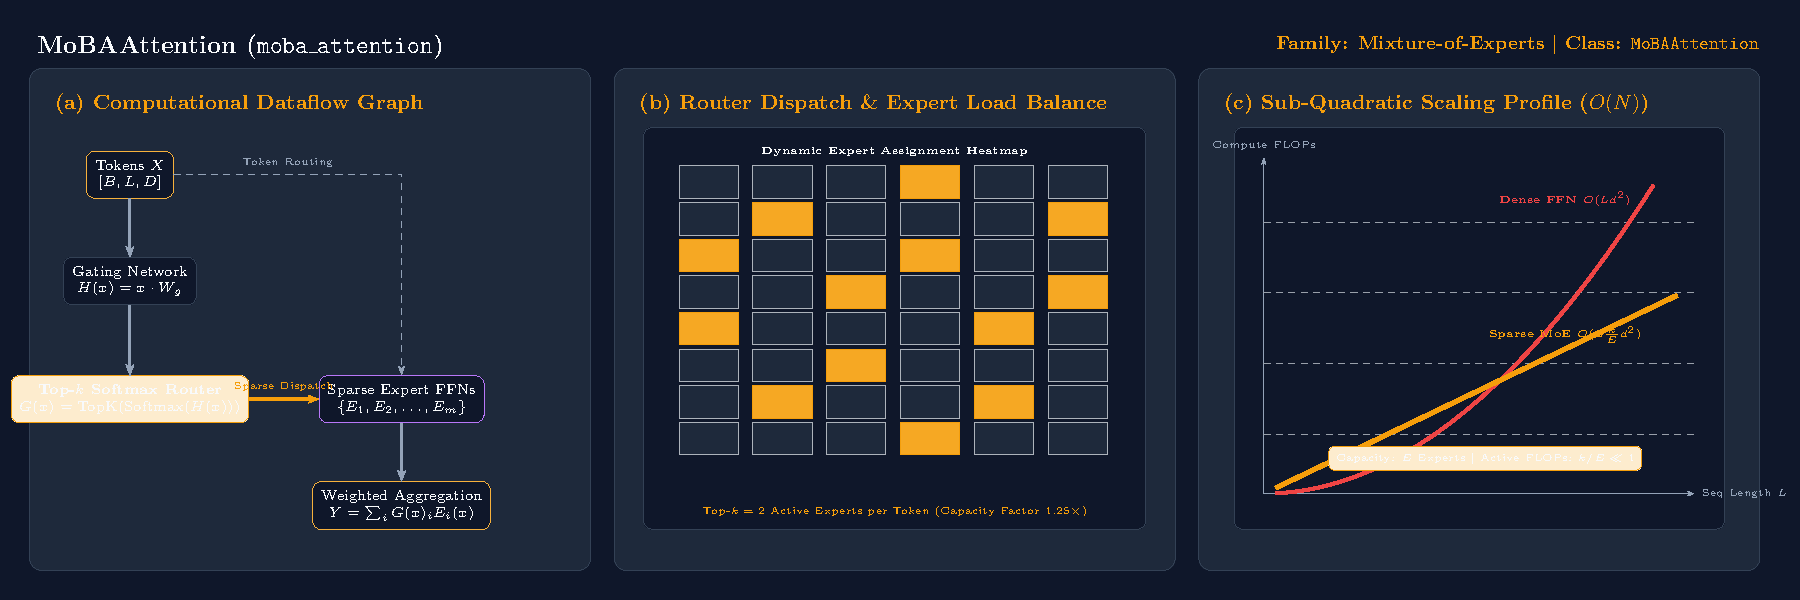
\includegraphics[width=0.98\textwidth]{figures/catalog_visuals/module_moba_attention.pdf}
    \caption{\textbf{Comprehensive 3-Panel Architectural Characterization for MoBAAttention (\texttt{moba\_attention})}. (a) Computational Dataflow Graph and Operator Connectivity; (b) Structural Dynamics, Spectral Decay, and Heatmap; (c) Theoretical Scaling Profile against Quadratic Baselines.}
    \label{fig:module_moba_attention}
\end{figure}

\vspace{1.0em}
\hrule
\vspace{1.0em}
